\section{Introducción}
\subsection{Conceptos claves}

\subsubsection{Computación Paralela}

La computación paralela es el uso simultáneo de más de un procesador para resolver
un problema.
La computación paralela es una técnica de programación en la que muchas instrucciones se ejecutan simultáneamente. Se basa en el principio de que los problemas grandes se pueden dividir en partes más pequeñas que pueden resolverse de forma concurrente.

\subsubsection{MPI}
MPI es un estándar de programación en paralelo mediante paso
de mensajes que permite crear programas portables y eficientes.
El paso de mensajes es una técnica empleada en programación concurrente para aportar sincronización entre procesos y permitir la exclusión mutua.

Su principal característica es que no precisa de memoria compartida, por lo que es muy importante en la programación de sistemas distribuidos. 

Al arrancar una aplicación se lanzan en paralelo n copias del mismo programa(procesos), facilita legibilidad y mantenimiento Distinción del código a ejecutar por cada uno: mediante el id del proceso

\begin{figure}[H]
    \centering
  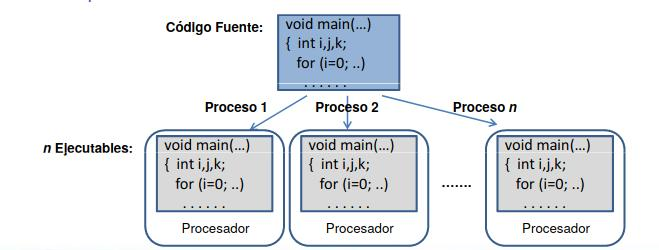
\includegraphics[width=0.7\textwidth]{images/mpi_estructure.jpg}
  \caption{Estructura MPI}
  \label{esq}
\end{figure}


\subsubsection{NFS}

El Sistema de archivos de red (NFS) es una aplicación cliente / servidor que permite al usuario de una computadora ver y opcionalmente, almacenar y actualizar archivos en una computadora remota como si estuvieran en la computadora del usuario. El protocolo NFS es uno de los varios estándares del sistema de archivos distribuidos para el almacenamiento conectado a la red (NAS).

NFS permite al usuario o administrador del sistema montar (designar como accesible) todo o una parte de un sistema de archivos en un servidor. Los clientes pueden acceder a la parte del sistema de archivos que está montada con los privilegios asignados a cada archivo (solo lectura o lectura-escritura). NFS utiliza llamadas a procedimiento remoto (RPC) para enrutar solicitudes entre clientes y servidores. \url{https://searchenterprisedesktop.techtarget.com/definition/Network-File-System}

\subsubsection{Geant4}
Geant4 es un conjunto de herramientas para la simulación del paso de partículas a través de la materia. Sus áreas de aplicación incluyen física de alta energía, nuclear y aceleradora, así como estudios en medicina y ciencia espacial.

\subsubsection{G4mpi}

G4MPI es una interfaz nativa con bibliotecas MPI. El directorio contiene una biblioteca Geant4 UI y un par de ejemplos paralelos. Al usar esta interfaz, las aplicaciones de los usuarios se pueden paralelizar con diferentes bibliotecas compatibles con MPI, como OpenMPI, LAM / MPI, MPICH2, etc.

\subsection{Metodología y Esquema general de la arquitectura}

\begin{enumerate}
    \item Hacer hostst/cluster del entorno MPI 
    \item Lanzar el entorno de ejecución de MPI.
    \item Ejecutar aplicación mpirun -np 8 myapp
    \item Ejecutar comandos MPI G4UI, ubicados en /mpi/
    
\end{enumerate}


\begin{figure}[H]
    \centering
  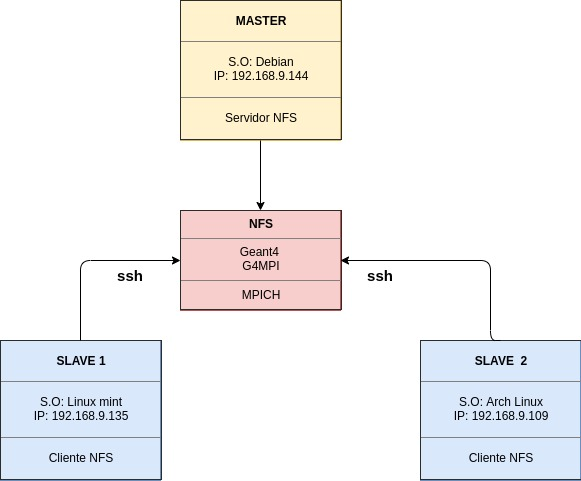
\includegraphics[width=0.7\textwidth]{images/EsquemaGeneral.jpg}
  \caption{Esquema}
  \label{esq}
\end{figure}


\newpage